\documentclass[12pt]{article}
\usepackage{graphicx}
\usepackage[none]{hyphenat}
\usepackage{graphics}
\usepackage{refstyle}
\usepackage[english]{babel}
\usepackage{amsmath}
\usepackage{caption}
\usepackage[parfill]{parskip}
\usepackage{hyperref}
\usepackage{booktabs}
\usepackage{float}
\usepackage{physics}
\usepackage{tasks}
\usepackage{listings}
\usepackage[utf8]{inputenc}
\graphicspath{{storage/self/primary/Download/maths/figs}}
\usepackage{color}
\usepackage{array}   
\usepackage{longtable}
\usepackage{calc}  
\usepackage{multirow}
\usepackage{hhline} 
\usepackage{ifthen}
\usepackage{array}
\newcommand{\mydet}[1]{\ensuremath{\begin{vmatrix}#1\end{vmatrix}}}
\providecommand{\brak}[1]{\ensuremath{\left(#1\right)}}
\providecommand{\norm}[1]{\left\lVert#1\right\rVert}
\newcommand{\solution}{\noindent \textbf{Solution: }}
\newcommand{\myvec}[1]{\ensuremath{\begin{pmatrix}#1\end{pmatrix}}}
\let\vec\mathbf

\begin{document}
\begin{center}
 \section*{\textbf{Class 12}}
 \subsection*{Chapter 10 - Vector Algebra}
\end{center}
This is question 18 from exercise 10.5 \\
\begin{enumerate}
\item  The value of  $\hat{i} \cdot (\hat{j} \times \hat{k})$  + $\hat{j} \cdot (\hat{i} \times \hat{k})$ + $\hat{k} \cdot (\hat{i} \times \hat{j} )$ is
 \begin{tasks}(4)
    \task $0$ 
    \task $-1$ 
    \task $1$ 
    \task $3$  
  \end{tasks}
\end{enumerate}
\textbf{Solution:}
The Directional vectors of $x,y$ and $z$ axes are given respectively 
\begin{align}
  \vec{e_1} =\myvec{1\\0\\0},\vec{e_2}=\myvec{0\\1\\0},\vec{e_3} =\myvec{0\\0\\1}
\end{align}
Now,\\
\begin{center} 
$\myvec{1\\0\\0}\cdot (\myvec{0\\1\\0} \times \myvec{0\\0\\1})$  + $\myvec{0\\1\\0} \cdot (\myvec{1\\0\\0} \times \myvec{0\\0\\1})$ + $\myvec{0\\0\\1} \cdot (\myvec{1\\0\\0} \times \myvec{0\\1\\0} )$ \\
= $\myvec{1\\0\\0} \cdot (\myvec{1\\0\\0}) + \myvec{0\\1\\0} \cdot (-\myvec{0\\1\\0}) + \myvec{0\\0\\1} \cdot (\myvec{0\\0\\1})$ \\
= $\myvec{1\\0\\0} \cdot \myvec{1\\0\\0} - \myvec{0\\1\\0} \cdot \myvec{0\\1\\0} + \myvec{0\\0\\1} \cdot \myvec{1\\0\\0}$ \\
\end{center}
\fbox{\begin{minipage}{15em}
$\myvec{1\\0\\0} \cdot \myvec{1\\0\\0} = |\myvec{1\\0\\0}| |\myvec{1\\0\\0}| \cos{0} $ \\
                       = $ 1 \times 1 \times 1 $ \\
                       = $ 1 $ \\
similarly, $ \\myvec{0\\1\\0} \cdot \myvec{0\\1\\0} = \myvec{0\\0\\1} \cdot \myvec{0\\0\\1} = 1$
\end{minipage}}
\begin{center}
    = $ 1 - 1 + 1 $\\
    =$1$\\
\end{center}
So, option (c) is correct.

\begin{figure}[H]
        \centering
  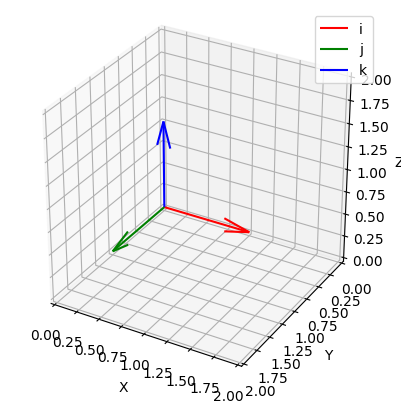
\includegraphics[width=\columnwidth]{figs/unit_vec.png}
                \label{fig:12/10/5/18}
         \caption{fig:1}
               \end{figure}
\end{document}
